\subsection{Equivariance Ablation}
\label{AblationEquivariance}
To test the impact of restricting the equivariance of RENI++ to $SO(2)$, we ran an ablation of models with $SO(3)$, $SO(2)$ and without equivariance at three sizes of latent code dimension $D$. For the model without equivariance, we augmented the dataset with rotations of the images at increments of $0.785 \text{rad}$ for a training dataset size of $13,384$ images. The $SO(2)$ case performs best for all latent code sizes except $D = 27$, and the $SO(2)$ model outperforms the model trained purely using augmentation whilst using significantly less data. Results are shown in Table \ref{tab:comparison_equivariance}.

\begin{table}\centering
\vspace{-0.37cm} % Adjust -0.5cm as needed
\begin{tabular}{@{}c ccc@{}}\toprule
D & None & SO(2) & SO(3)   \\
\midrule
$27$  & 17.23 & 18.02 & \textbf{18.09} \\
$108$ & 20.00 & \textbf{20.87} & 20.11 \\
$147$ & 20.81 & \textbf{21.13} & 20.66 \\
$300$ & 21.41 & \textbf{22.10} & 21.12 \\
\bottomrule
\end{tabular}
\caption{Mean PSNR on the test set for models with varying levels of equivariance.}
\label{tab:comparison_equivariance}
\end{table}

\subsection{Additional Render}
RENI++ environment maps can be exported and used within traditional graphics pipelines. Figure \ref{fig:blender} shows comparison renders between ground truth and RENI++ environment maps rendered within the computer graphics software tool Blender. The results are very similar with only minor differences in the highly specular regions.

\begin{figure}
    \vspace{-0.4cm} % Adjust -0.5cm as needed
    \centering
    \makebox[\columnwidth]{%
        \begin{tikzpicture}
        \node (img) {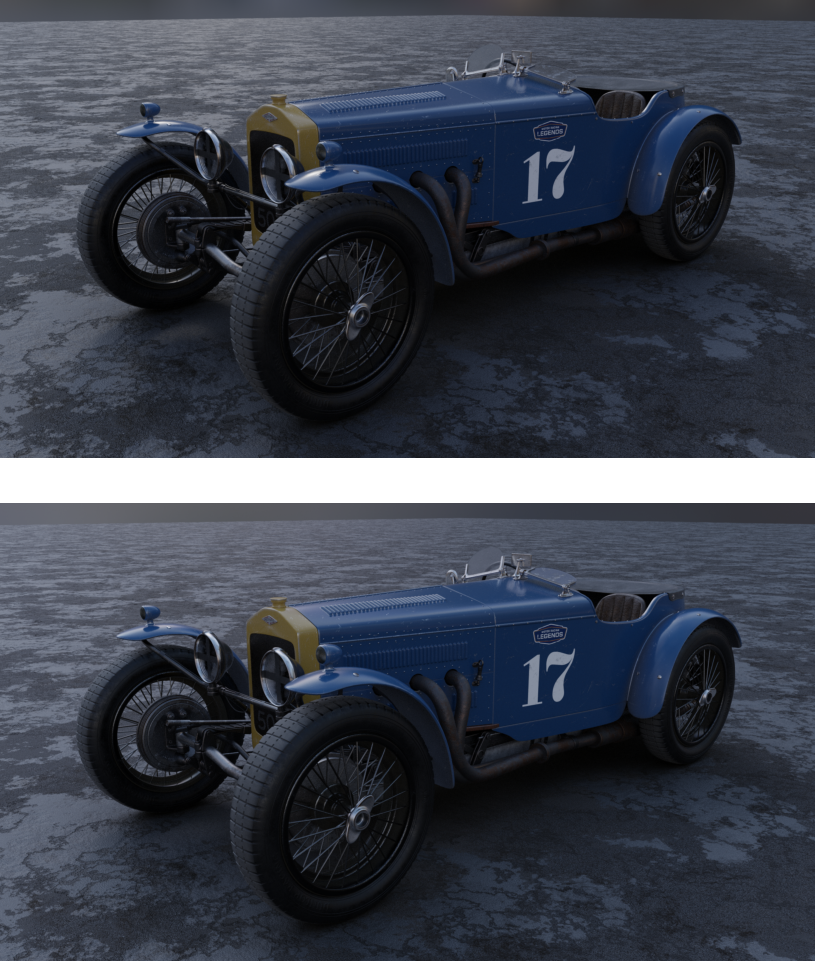
\includegraphics[width=0.95\columnwidth]{Figures/blender_render.pdf}};
        \node at (0.0, 5.2) {\scriptsize Ground Truth};
        \node at (0.0, -0.05) {\scriptsize RENI++};
        \end{tikzpicture}
    }
    \caption{Blender renders showing comparison between ground truth and RENI++ environment maps.}
    \label{fig:blender}
\end{figure}